\documentclass[dvipsnames]{article}

\usepackage{tikz}

%%%%%%%%%%%%%%%%%%%%%%%%%%%%%%%% TIKZ STYLES
\tikzstyle{every node}=[font=\scriptsize]

\tikzset{RootStyle/.style = {
						shape          = circle,
			      draw           = red!50!black!50,
			      thick,
			      top color      = white,
			      bottom color   = red!50!black!20,
			      text           = black,
			      inner sep      = .2pt,
			      outer sep      = 0pt,
			      minimum size   = 2.5 mm}
						}

\tikzset{VertexStyle/.style = {
						shape          = circle,
			      draw           = black!50,
			      top color      = white,
			      bottom color   = black!20,
			      text           = black,
			      inner sep      = .2pt,
			      outer sep      = 0pt,
			      minimum size   = 1.75 mm}
						}

\tikzset{EdgeStyle/.style   = {thick,<->}}

\tikzset{LabelStyle/.style =   {
				  text           = black,
				  inner sep      = .2pt,
				  outer sep      = 1pt,
				  font           =\scriptsize,
				  minimum size   = 2.15 mm}
					}

\begin{document}

\begin{figure}
			\begin{center}
					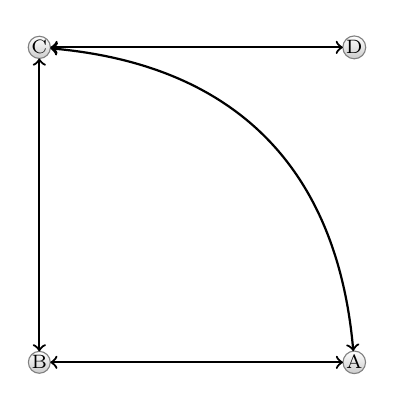
\begin{tikzpicture}[xscale=2,yscale=2,auto]
							\draw (2,0) node[VertexStyle]   (A) { A };
							\draw (0,0) node[VertexStyle] (B) { B };
							\draw (0,2) node[VertexStyle]   (C) { C };
							\draw (2,2) node[VertexStyle]   (D) { D };

							\draw[EdgeStyle]				(B) to node[LabelStyle]{}	(A);
							\draw[EdgeStyle,bend left=40,looseness=1.1]    	(C) to node[LabelStyle]{}   	(A);
							\draw[EdgeStyle] 	(C) to node[LabelStyle]{}     	(B);
							\draw[EdgeStyle]  	(C) to node[LabelStyle]{} 		(D);
							%\draw[EdgeStyle,bend left=40,looseness=1.1]   	(A) to node    	(sink);

					\end{tikzpicture}
			\end{center}
	\caption{Un super graphe en TiKz}
	\label{fig:tikzminimal}
\end{figure}

\end{document}